\section{Test concorrenziale}\label{sec:test_concorrenziale}

In questo Test empirico si vuole vedere come Elixir
si comporta all'aumentare dei processi.

In particolare si sono scelti una lista di campioni
di processi "processes" da utilizzare per ogni test, per ogni
valore della lista processes
si eseguono una serie prodotti che vanno da 500 prodotti
a 100000 prodotti con uno step di 500.

Si calcola quindi il tempo impiegato per ogni campione
e si stampa il campione sul un file csv da poter analizzare
ed interpretare su Matlab.
I campioni di processi da creare per ogni test
sono riportati nella lista:
\begin{lstlisting}[language=none]
processes = [1,2,3,4,5,6,7,8,16,32,64,128,256]
\end{lstlisting}

\subsection{Implementazione del Test}

Il codice Elixir che esegue il test è
implementato nel modulo Elixir ConcurrentTask e
riportato nel Listing \ref{lst:concurrent_task}.


\begin{lstlisting}[language=elixir, caption={Test concorrenziali},captionpos=b,
	label={lst:concurrent_task}]
defmodule ConcurrentTask do
  require Logger
  import MyFile


  def compute_products(productsnumber) do
    for _i <- 1..productsnumber do
  	1 * 1000
    end
  end


  def run do
    processes = [1, 2, 3, 4, 5, 6, 7, 8, 16, 32, 64, 128, 256]
    productsnumber = 100_000
    step = 500
  
    for proc <- processes do
  	Logger.info("processes #{proc} and #{System.schedulers} scheduler")
  	for comp <- 500..productsnumber//step do
  	  {:ok, _time} = parallel_operations(comp, proc)
  	end
    end
  end

	def parallel_operations(productsnumber, processnumber) do
  
    	#divide the products number to assign to each process
		temp = trunc(productsnumber / processnumber)
  		# compute the rest to compute to restTask
  		rest = rem(productsnumber , processnumber)
  
  		{time, _result} =
  	  	:timer.tc(
	  		fn ->
  		  	tasks =
  				for _i <- 1..processnumber do
  			  	Task.async(fn -> compute_products(temp) end)
  				end
  		  	restTask = Task.async(fn -> compute_products(rest) end)
  
  		  	# Aspetta di finire ogni task per ottenere i risultati
  		  	for task <- tasks do
  				Task.await(task, :infinity)
  		  	end
  		  	Task.await(restTask, :infinity)
  			end,
  			[],
  			:microsecond
  	  	)
  	  	writeData2File(time,processnumber,productsnumber)
  	  	{:ok,time}
	end

	def writeData2File(time,processnumber,productsnumber) do
  	available_scheduler = 
		:erlang.system_info(:logical_processors_available)

	scheduler = System.schedulers()

  		data = [
		"#{scheduler},",
		"#{available_scheduler},",
		"#{time},",
		"#{processnumber},",
		"#{productsnumber},",
		"#{time/productsnumber}\n"
  	]

	# scrittura risultato su file
	write(data)
  	{:ok, time}
	end
end
  
\end{lstlisting}

La funzione write che si occupa della scrittura
dei dati su file si trova nel modulo MyFile riportato nel
Listing \ref{lst:MyFile}.


\begin{lstlisting}[language=elixir, caption={Modulo MyFile},
	captionpos=b,label={lst:MyFile}]
defmodule MyFile do
	def write(data,file_path \\ "./File/test.csv") do
		{:ok, file} = File.open(file_path, [:write,:append])
		IO.write(file, data)
    	File.close(file)
	end 
end
\end{lstlisting}

Il modulo Task utilizzato fornisce un modo per eseguire
una funzione in background e recuperarne il valore
restituito in un secondo momento.
Il modulo Task fornito è
implementato utilizzando la primitiva spawn\_link discussa
in precedenza.

%++++++++++++++++++++++++++++++++++++++++++++++++++++++++++

\subsection{Esecuzione Test}

Si è creato uno script per l'ambiente interattivo iex per l'avvio
della funzione voluta riportato nel Listing \ref{lst:script_iex}

\begin{lstlisting}[language=none,captionpos=b,
	caption={Script iex per l'avvio dei test},
	label={lst:script_iex}]
:code.purge(ConcurrentTask)
:code.delete(ConcurrentTask)
c("lib/concurrent_task.ex")
ConcurrentTask.run
System.halt
\end{lstlisting}
	


Il test fornito è stato eseguito più volte aumentando
gli scheduler allocati all'avvio dell'istanza della VM.
Si è scritto un semplice script in bash per eseguire
i vari test all'aumentare degli scheduler allocati, lo script
è riportato nel Listing \ref{lst:script_bash}.
La macchina virtuale di default viene allocata con 8
scheduler, si avvia con il numero di scheduler voluti
impostando il flag --erl "+S1".

\begin{lstlisting}[language=none,captionpos=b,
	caption={Script bash per l'avvio dei test},
	label={lst:script_bash}]

#!/bin/bash

iex --erl "+S 1" --dot-iex "runTest.iex" -S mix
iex --erl "+S 2" --dot-iex "runTest.iex" -S mix
iex --erl "+S 3" --dot-iex "runTest.iex" -S mix
iex --erl "+S 4" --dot-iex "runTest.iex" -S mix
iex --erl "+S 5" --dot-iex "runTest.iex" -S mix
iex --erl "+S 6" --dot-iex "runTest.iex" -S mix
iex --erl "+S 7" --dot-iex "runTest.iex" -S mix
iex --erl "+S 8" --dot-iex "runTest.iex" -S mix
iex --erl "+S 9 +sbt db" --dot-iex "runTest.iex" -S mix
iex --erl "+S 10 +sbt db" --dot-iex "runTest.iex" -S mix
iex --erl "+S 11 +sbt db" --dot-iex "runTest.iex" -S mix
iex --erl "+S 12 +sbt db" --dot-iex "runTest.iex" -S mix
iex --erl "+S 13 +sbt db" --dot-iex "runTest.iex" -S mix
iex --erl "+S 14 +sbt db" --dot-iex "runTest.iex" -S mix
iex --erl "+S 15 +sbt db" --dot-iex "runTest.iex" -S mix
iex --erl "+S 16 +sbt db" --dot-iex "runTest.iex" -S mix
	
\end{lstlisting}

Per avviare lo script eseguire i comandi:
\begin{lstlisting}[language=none]
# solo la prima volta alla creazione del file
chmod +x <directory-path>/runtest.sh 

.<directory-path>/runtest.sh
\end{lstlisting}

Una volta avviati i test verrà creato un file .csv da
analizzare con Matlab, i valori presenti nel file
assumono la forma:

\begin{lstlisting}[language=none,captionpos=b,
	caption={File csv} \label{lst:formatocsv}]
N\_Scheduler,N\_Available_Scheduler,Time,N\_Processes,N\_Products
1,8,39,1,500
1,8,24,1,1000
1,8,19,1,1500
1,8,20,1,2000
1,8,22,1,2500
.....
\end{lstlisting}


%++++++++++++++++++++++++++++++++++++++++++++++++++
\subsection{Analisi Matlab}

In Matlab viene analizzato il file .csv risultante dal
test, stampando un grafico per ogni numero di scheduler utilizzato.
Lo script Matlab è riportato nel Listing \ref{lst:analisi_matlab}.

\begin{lstlisting}[language=none,captionpos=b,
	caption={File csv},label={lst:analisi_matlab}]
N\_Scheduler,N\_Available_Scheduler,Time,N\_Processes,N\_Products
opts = detectImportOptions('/home/nico/project/tesi/analisi_elixir/File/test_concorrenza2.csv');
opts.DataLine = 2;
data = readtable('/home/nico/project/tesi/analisi_elixir/File/test_concorrenza2.csv', opts);

colors = [
    255 0   0   % Red
    0   255 0   % Green
    0   0   255 % Blue
    255 255 0   % Yellow
    0   255 255 % Cyan
    255 0   255 % Magenta
    128 128 128 % Gray
    255 128 0   % Orange
    128 0   128 % Purple
    0   128 128 % Teal
    128 128 0   % Olive
    255 165 0   % Orange (Web Color)
    0   255 127 % Spring Green
    ];
colors = colors / 255;
processes = [1,2,3,4,5,6,7,8,16,32,64,128,256];

for n = 1:16

    figure;

    for i = 1:length(processes)

        num_processes = processes(i);

        % Filtra i dati per N_Processes = 1 e N_Products = 1
        filteredData = ... 
		data(data.N_Processes == num_processes ... 
		     & data.N_Scheduler==n,:);

        filteredTime = ... 
		(filteredData.Time ./filteredData.N_Products);
        plot(filteredData.N_Products, filteredTime,... 
		     'Color', colors(i, :));

        hold on

    end
    xlabel('N_Products');
    ylabel('Time/Products');

    title('Grafico per n. Scheduler: ',n);


    legend('1 process','2 processes','3 processes','4 processes', ...
        '5 processes','6 processes','7 processes','8 processes', ...
        '16 processes','32 processes','64 processes',... 
		'128 processes','256 processes');
end
\end{lstlisting}

Lo script Matlab stampa 16 grafici, ne vengono riportati
tre, per l'esecuzione con 1 scheduler in figura \ref{fig:1_scheduler},
per 8 scheduler in figura \ref{fig:8_scheduler}
e per 16 \ref{fig:16_scheduler}.

\begin{figure}[!htp]
    \centering
    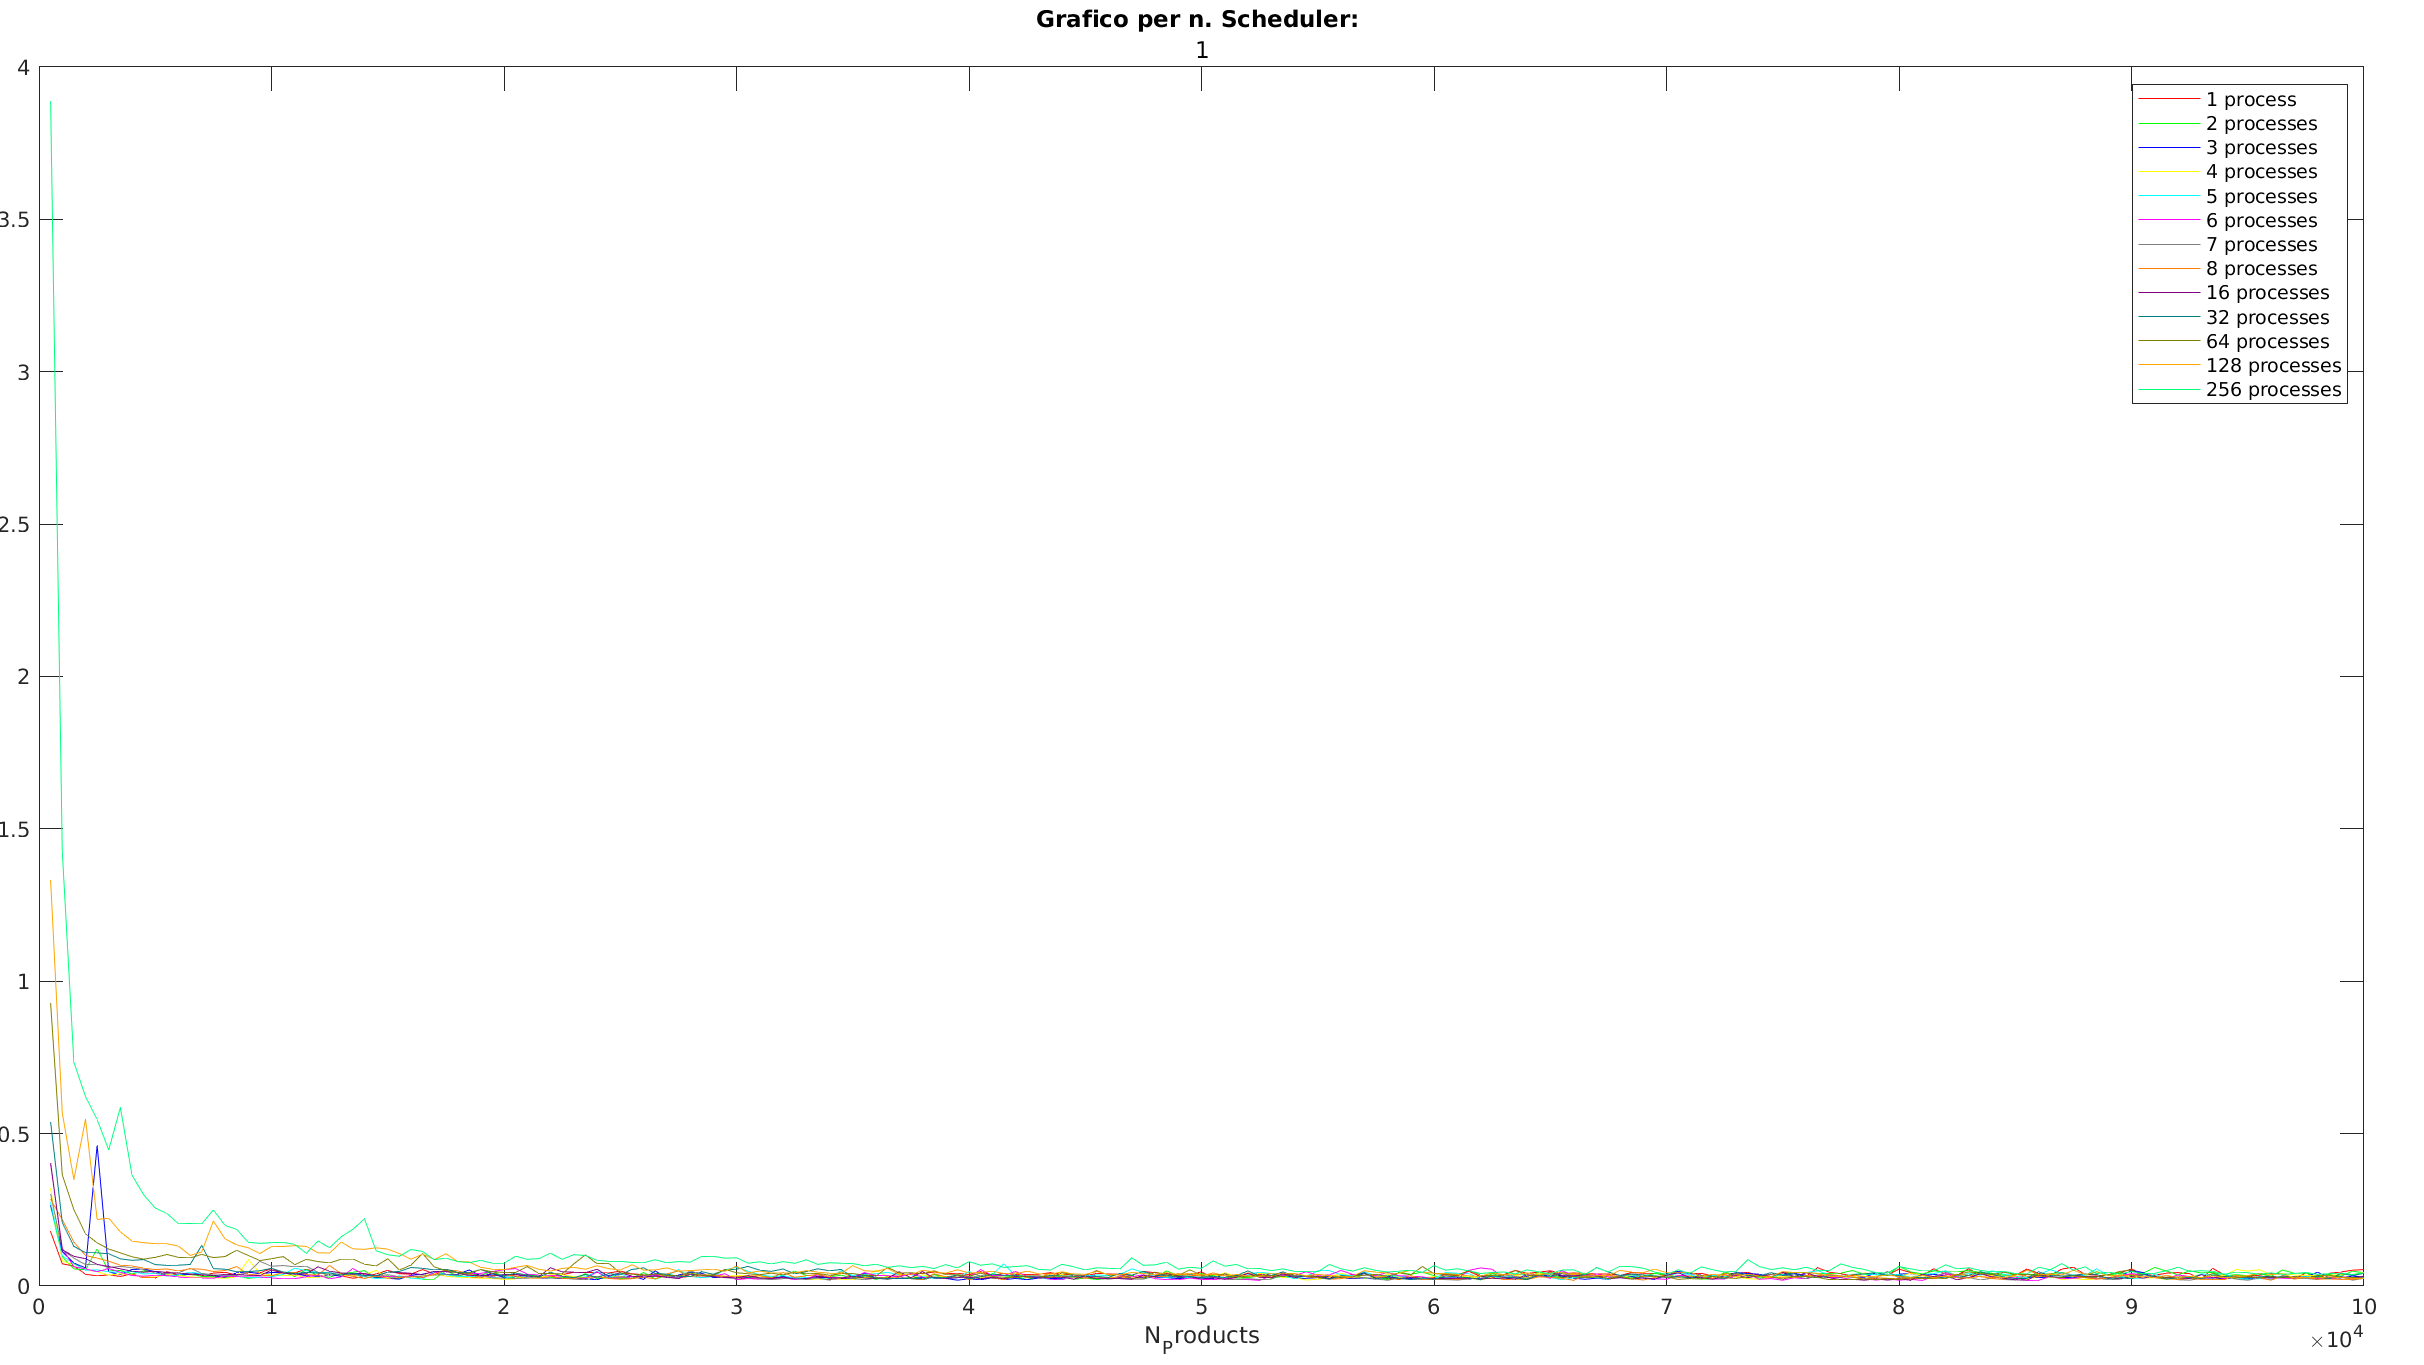
\includegraphics[keepaspectratio=true,scale=0.3]{images/matlab/1_scheduler.png}
	\caption{Grafico con 1 scheduler}
  	\label{fig:1_scheduler}
\end{figure}

\begin{figure}[!htp]
    \centering
    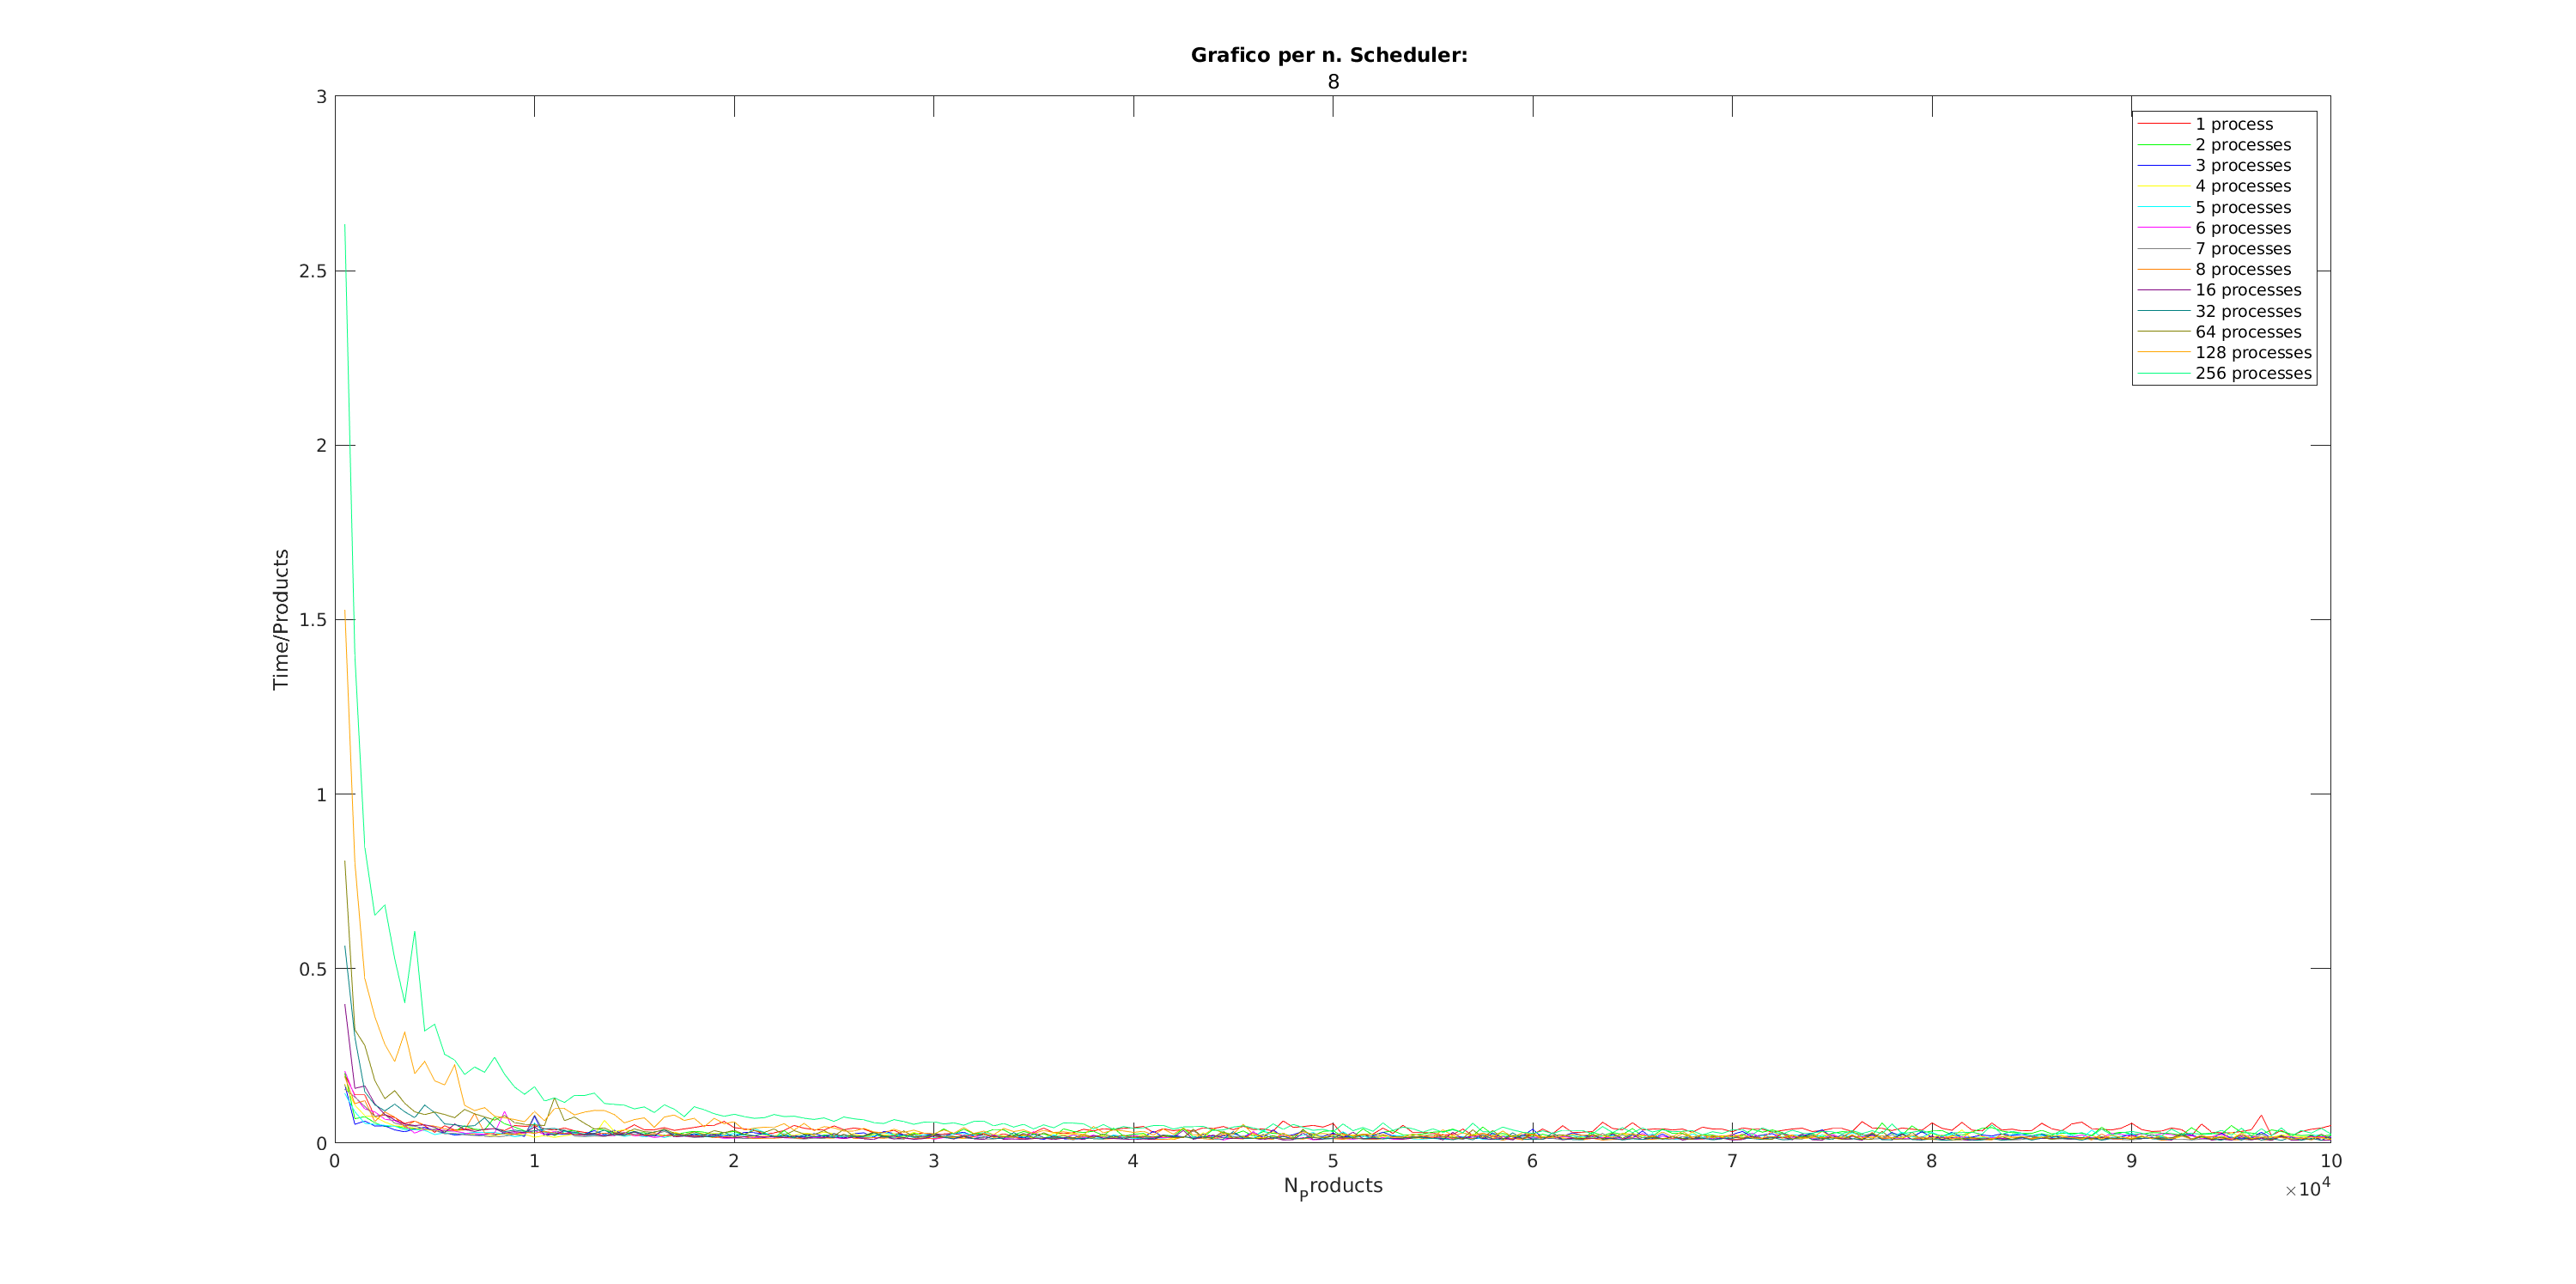
\includegraphics[keepaspectratio=true,scale=0.27]{images/matlab/8_scheduler.png}
	\caption{Grafico con 8 scheduler}
  	\label{fig:8_scheduler}
\end{figure}

\begin{figure}[!htp]
    \centering
    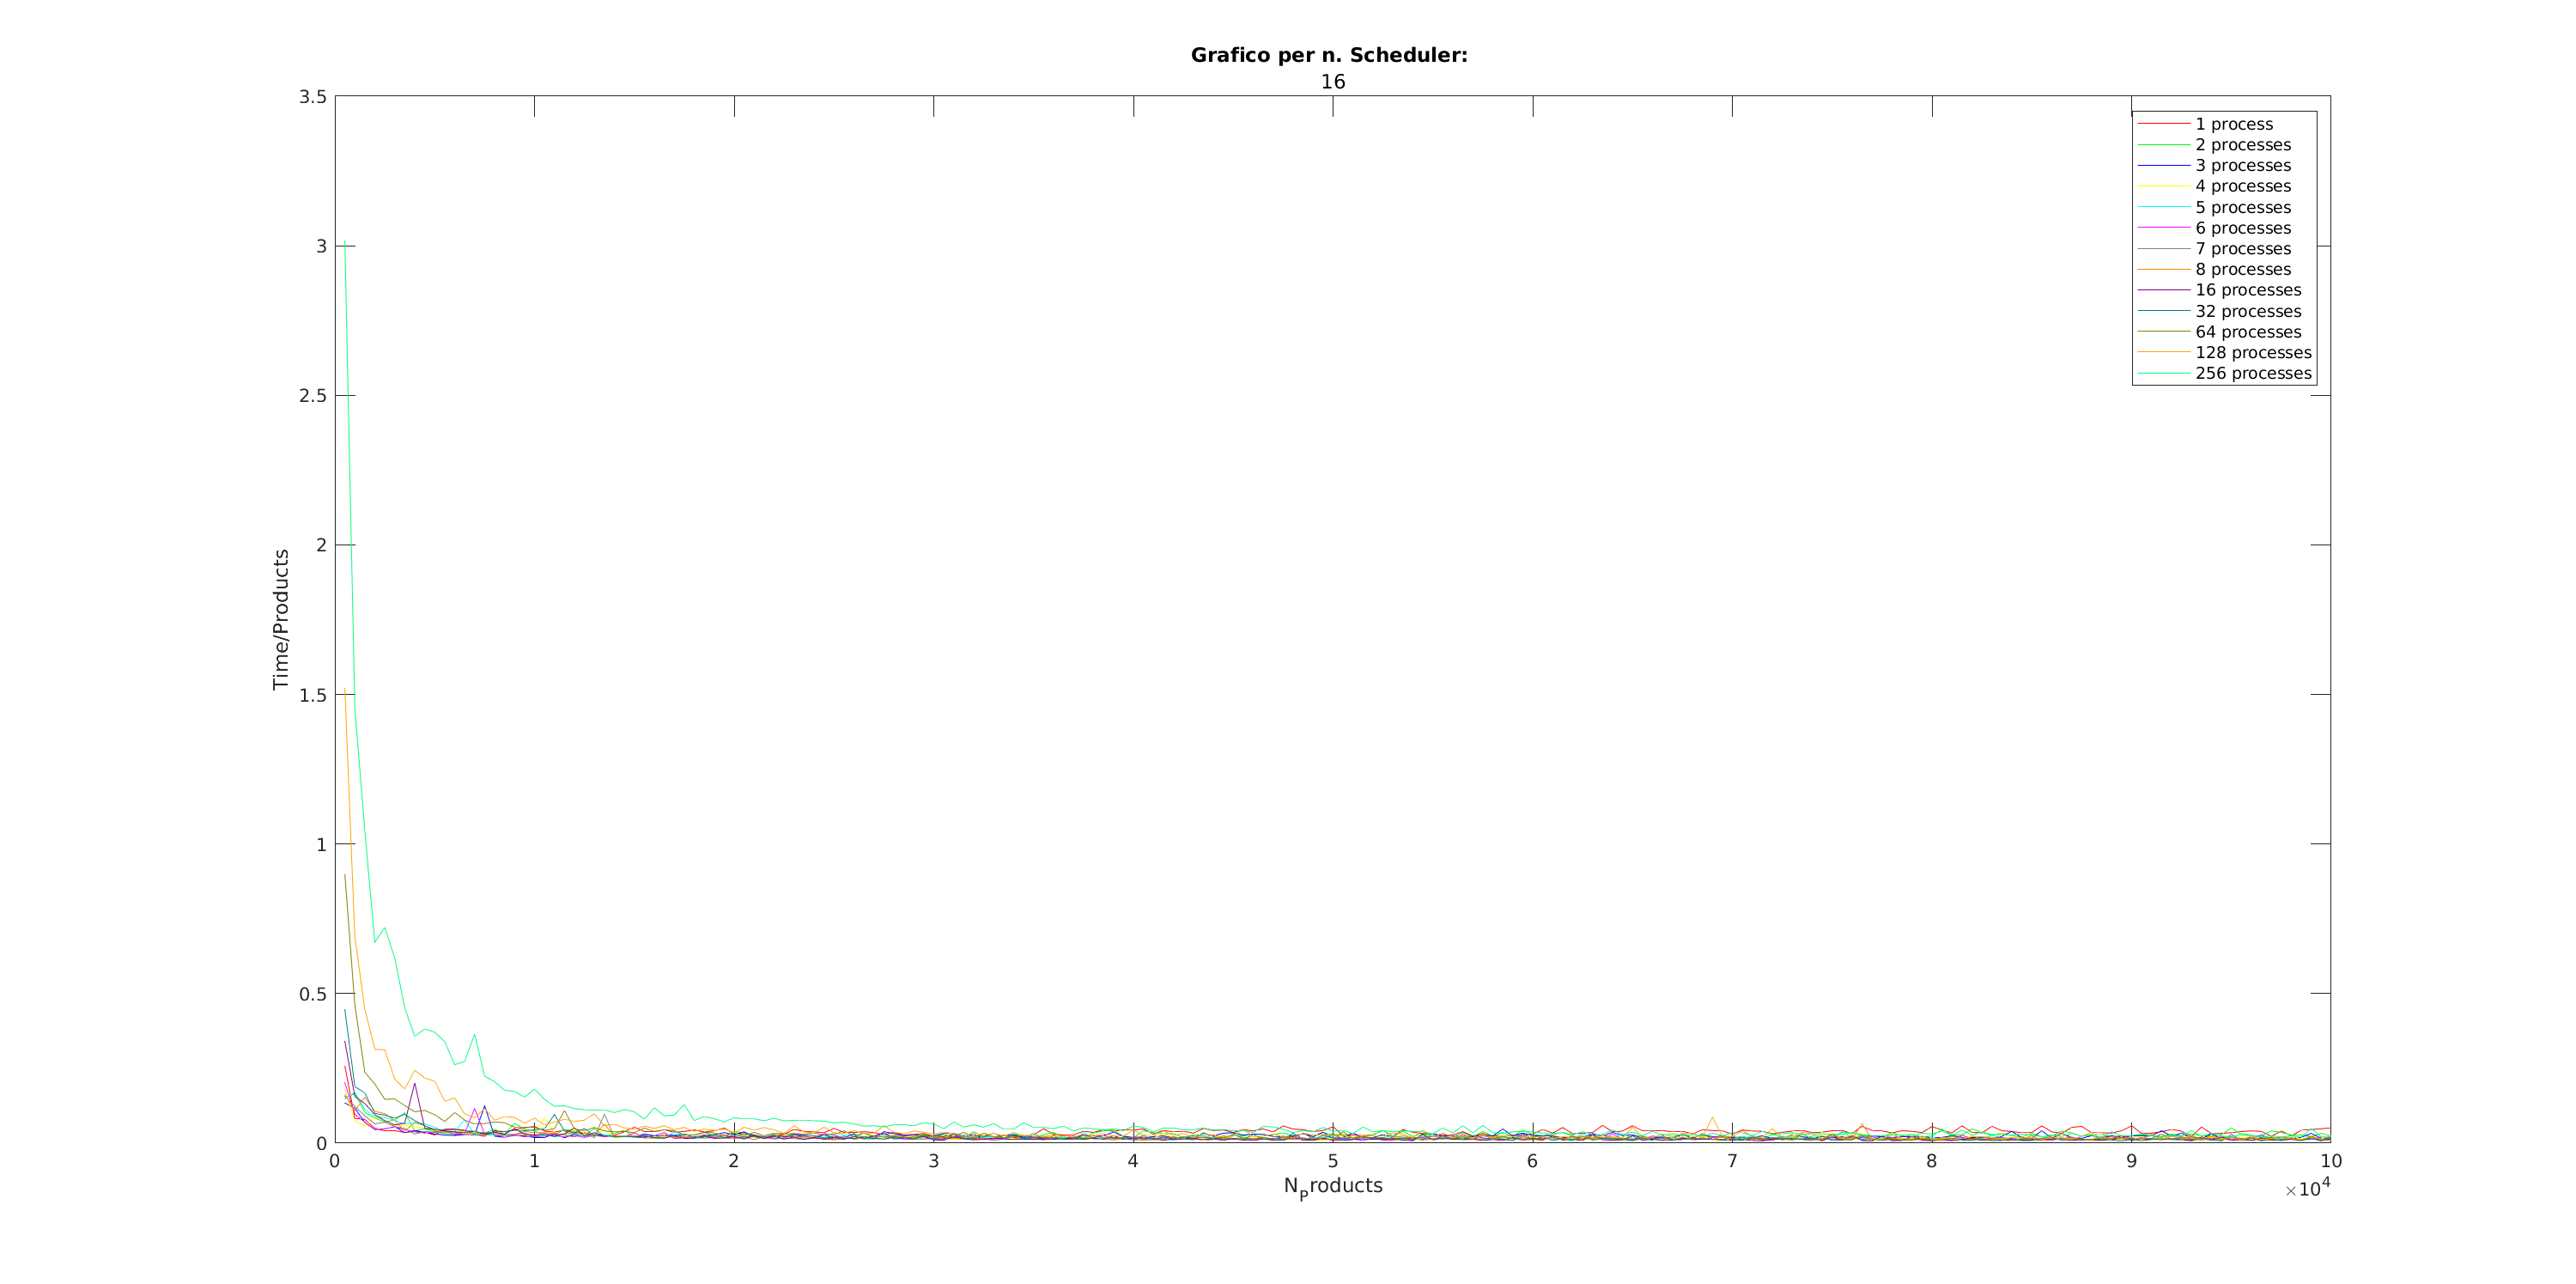
\includegraphics[keepaspectratio=true,scale=0.27]{images/matlab/16_scheduler.png}
	\caption{Grafico con 16 scheduler}
  	\label{fig:16_scheduler}
\end{figure}

I test risultano avere degli andamenti simi, possiamo notare che
con l'effettuazione di pochi prodotti, aumentare il numero dei processi
porta ad un degradamento delle performance, in quanto la VM si occupa più
di schedulare i processi che a fare prodotti.
Si nota però che per pochi processi, e poche operazioni, l'andamento
non è degradato. Come ci si aspetta però all'aumentare del numero di
prodotti, lo scheduling inizia ad avere meno importanza,
ed avere più processi porta a parallelizzare le operazioni ed a eseguirle
più velocemente.
Facendo uno zoom in un range che va da 88000 a 100000 prodotti come in
figura \ref{fig:zoom8}, si nota che le operazioni con un solo processo
hanno un andamento più alto, per esempio prendendo l'andamento più basso
del range di riferimento per un processo che si trova a 93000 prodotti,
eseguire 93000 prodotti risulta più efficiente se eseguiti con più di 3
processi.

Con un solo scheduler invece l'andamento con un processo risulta simile
a quello con più processi, ma il tempo impiegato con 8 scheduler risulta
in generale inferiore rispetto all'impiego di un solo scheduler, questo
fa capire che Erlang riesce a parallelizzare il numero di prodotti.


\begin{figure}[!htp]
    \centering
    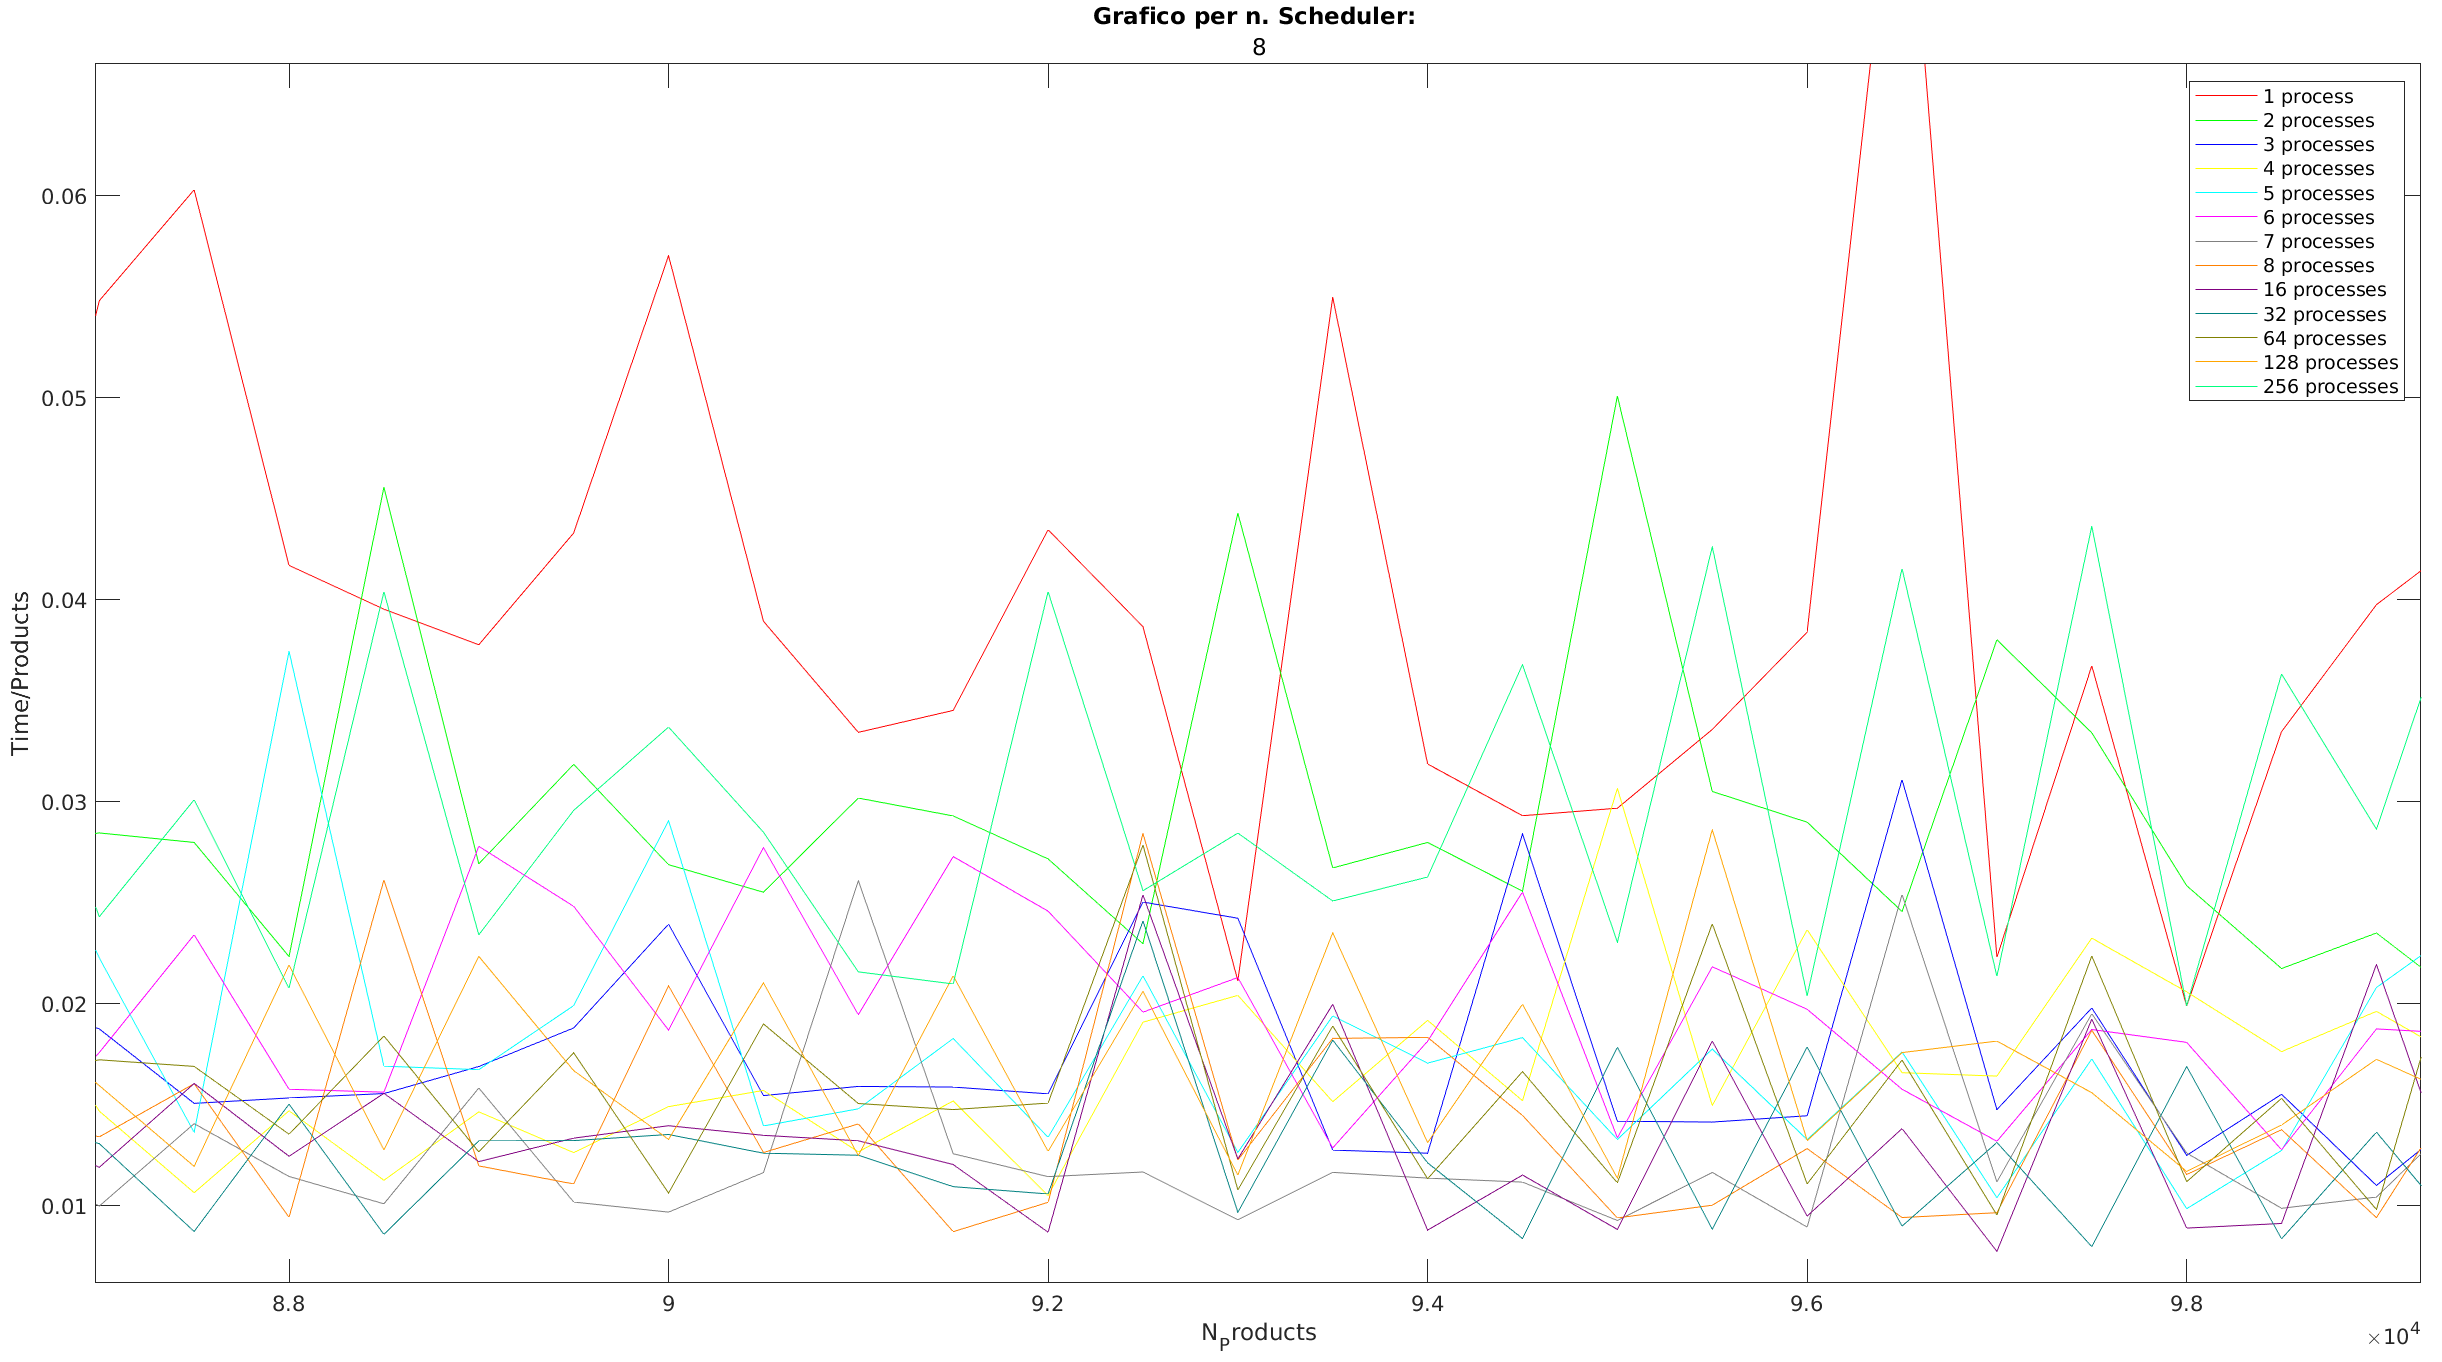
\includegraphics[keepaspectratio=true,scale=0.30]{images/matlab/zoom_8_crop.png}
	\caption{Zoom 88000-100000 prodotti con 8 scheduler}
  	\label{fig:zoom8}
\end{figure}



	